\documentclass[journal]{vgtc}       % preprint (journal style)

%% Uncomment one of the lines above depending on where your paper is
%% in the conference process. ``review'' and ``widereview'' are for review
%% submission, ``preprint'' is for pre-publication, and the final version
%% doesn't use a specific qualifier. Further, ``electronic'' includes
%% hyperreferences for more convenient online viewing.

%% Please use one of the ``review'' options in combination with the
%% assigned online id (see below) ONLY if your paper uses a double blind
%% review process. Some conferences, like IEEE Vis and InfoVis, have NOT
%% in the past.

%% Please note that the use of figures other than the optional teaser is not permitted on the first page
%% of the journal version.  Figures should begin on the second page and be
%% in CMYK or Grey scale format, otherwise, colour shifting may occur
%% during the printing process.  Papers submitted with figures other than the optional teaser on the
%% first page will be refused.

\usepackage{mathptmx}
\usepackage{graphicx}
\usepackage{times}
\usepackage{caption}
\usepackage{color}
\usepackage{bm}
\usepackage{amsmath}
\usepackage{microtype}
\usepackage[normalem]{ulem}

% options for TODO: either use red bold font for litle annotations (which do not work very well)

%\newcommand{\todo}[1]{\textcolor{red}{\textbf{TODO:} #1}}

% following commands are 'non standard' and not bundled with template, delete it problems occur
\usepackage{xargs}                      % Use more than one optional parameter in a new commands
\usepackage[pdftex,dvipsnames]{xcolor}  % Coloured text etc.
\usepackage[colorinlistoftodos,prependcaption,textsize=tiny]{todonotes}
\newcommand{\unsure}[1]{\todo[linecolor=red,backgroundcolor=red!25,bordercolor=red,inline]{#1}}
\newcommand{\change}[1]{\todo[linecolor=blue,backgroundcolor=blue!25,bordercolor=blue,inline]{#1}}
\newcommand{\info}[1]{\todo[linecolor=OliveGreen,backgroundcolor=OliveGreen!25,bordercolor=OliveGreen,inline]{#1}}
\newcommand{\improvement}[1]{\todo[linecolor=Plum,backgroundcolor=Plum!25,bordercolor=Plum,inline]{#1}}
\newcommand{\thiswillnotshow}[1]{\todo[disable,inline]{#1}}



\captionsetup[table]{justification=justified,singlelinecheck=false}
\captionsetup[figure]{justification=justified,singlelinecheck=false}

\vgtcinsertpkg



\title{Comvi - Comparative Visualization of Molecular Surfaces using Similarity-based Clustering}

\author{Wilhelm Buchm\"uller, Shoma Kaiser, Damir Ravilija, Enis ...}
\authorfooter{
\begin{tabular}{cccc}
  Wilhelm Buchmüller  & Shoma Kaiser & Enis .. . & Damir Rwilja  \\
 buch.willi@googlemail.com     & example@example.com       & example@example.com & example@example.com

\end{tabular}
}

%other entries to be set up for journal
%\shortauthortitle{Schmid \MakeLowercase{\textit{et\,al.}}: ProjINF for fun and profit}


\abstract{
The goal of this paper is to show the reader the abstract methods and concrete applications that were used to extract and compare features  and rank the similarity of the molecular protein maps. Further we present a new method of how the won data can be visualized on high resolution and large displays with a  The paper describes the process and the approaches that were taken to solve this task. 
} 


\keywords{Clustering, Similarity, feature extraction, Visualization, high-resolution display, Powerwall,MegaMol, VISUS}

%% ACM Computing Classification System (CCS).
%% See <http://www.acm.org/class/1998/> for details.
%% The ``\CCScat'' command takes four arguments.

\CCScatlist{ % not used in journal version
	\CCScat{Computer Graphics}{I.3.8}{Applications}{Molecular Dynamics Visualization}
	\CCScat{Simulation and Modeling}{I.6.6}{Simulation Output Analysis}{Molecular Dynamics Visualization}
	\CCScat{Computer Graphics}{I.3.7}{Three-Dimensional Graphics and Realism}{Raytracing}
}

\graphicspath{{pics/}}

%% Uncomment below to include a teaser figure.
%\teaser{
%\centering
%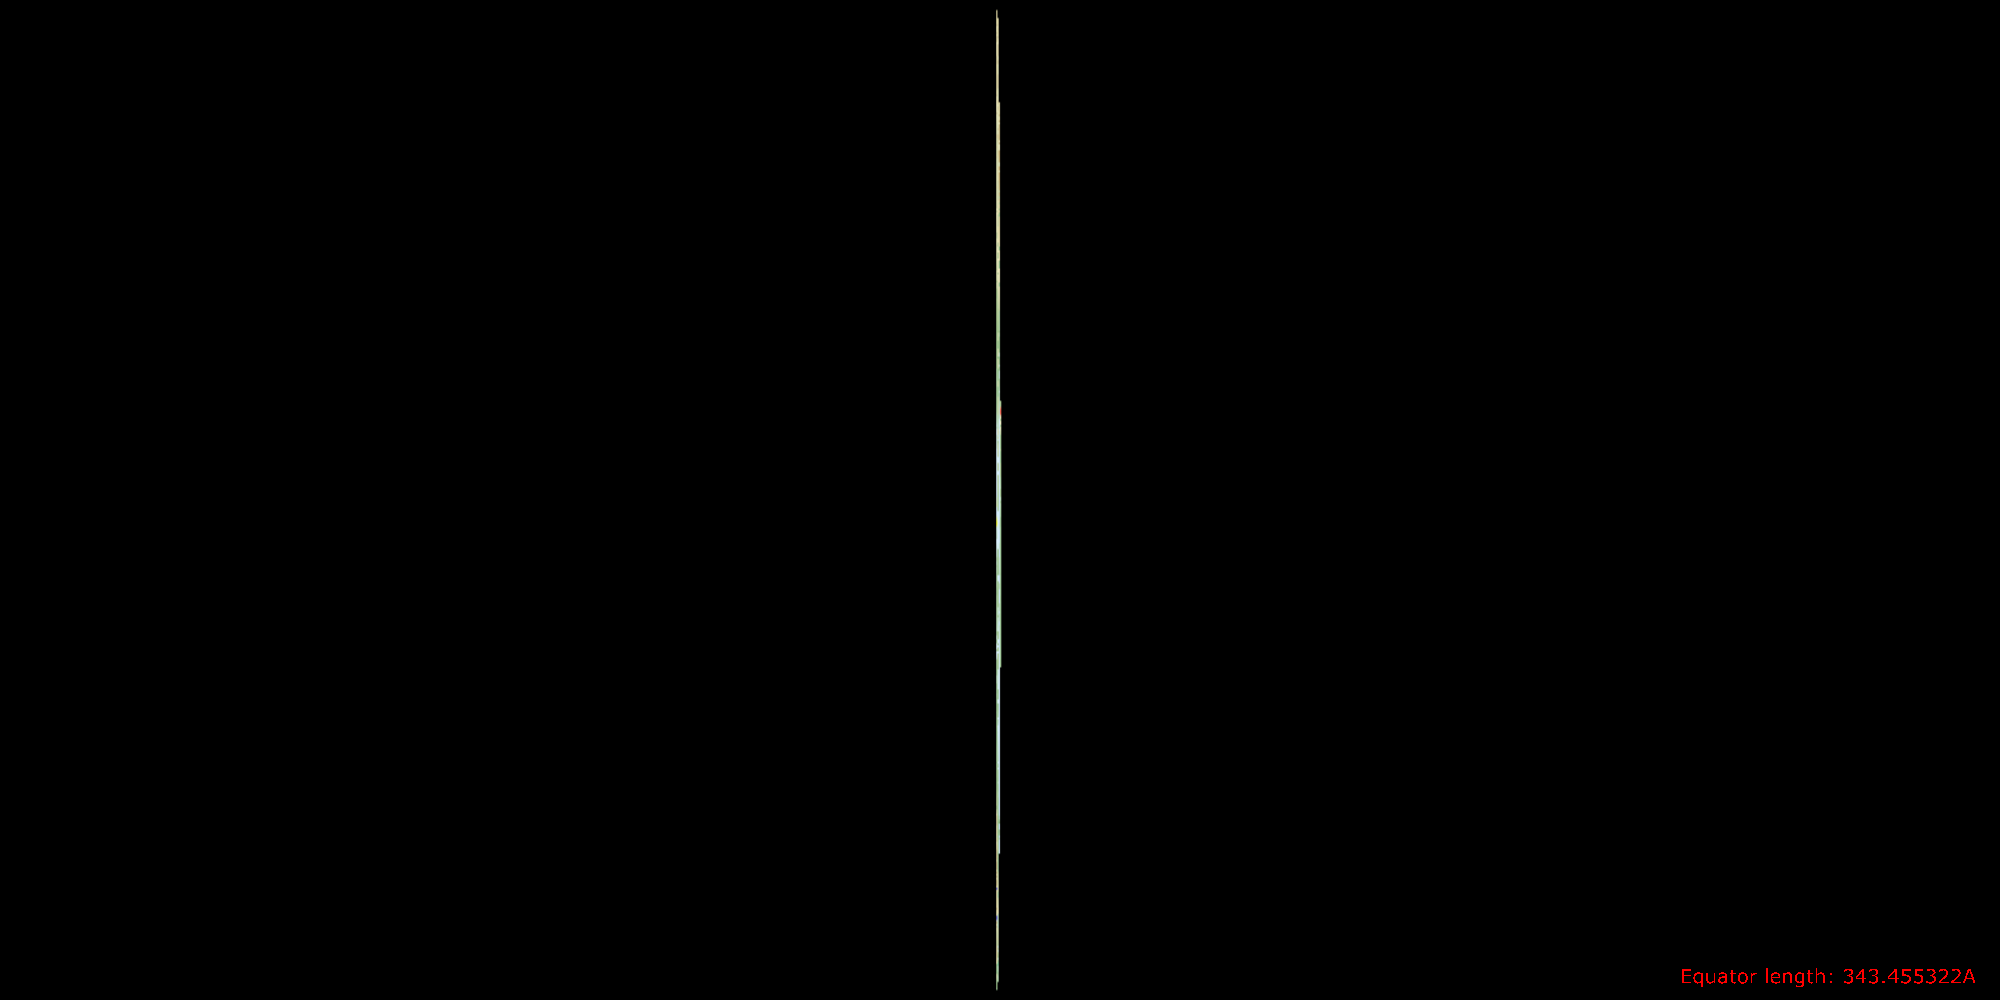
\includegraphics[width=12cm]{teaser}
%\caption{blah
%}\label{fig:teaser}
%}

%%%%%%%%%%%%%%%%%%%%%%%%%%%%%%%%%%%%%%%%%%%%%%%%%%%%%%%%%%%%%%%%
%%%%%%%%%%%%%%%%%%%%%% START OF THE PAPER %%%%%%%%%%%%%%%%%%%%%%
%%%%%%%%%%%%%%%%%%%%%%%%%%%%%%%%%%%%%%%%%%%%%%%%%%%%%%%%%%%%%%%%%

\begin{document}

%% The ``\maketitle'' command must be the first command after the
%% ``\begin{document}'' command. It prepares and prints the title block.

%% the only exception to this rule is the \firstsection command
\firstsection{Introduction}\label{sec:intro}
%
\maketitle
%
\firstsection{Introduction} %for journal use above \firstsection{..} instead
TODO's Beispiel Bitte entsprechend benutzen:
\unsure{unsure}
\change{change}
\info{info}
\improvement{improvement}
\thiswillnotshow{thiswillnotshow}
Over the span of 6 months the authors have
Ut wisi enim ad minim veniam, quis nostrud exerci tation ullamcorper suscipit lobortis nisl ut aliquip ex ea commodo consequat. Duis autem vel eum iriure dolor in hendrerit in vulputate velit esse

%-------------------------------------------------------------------------
\section{Related Work}\label{sec:relatedWork}

\begin{figure}
  \begin{center}
  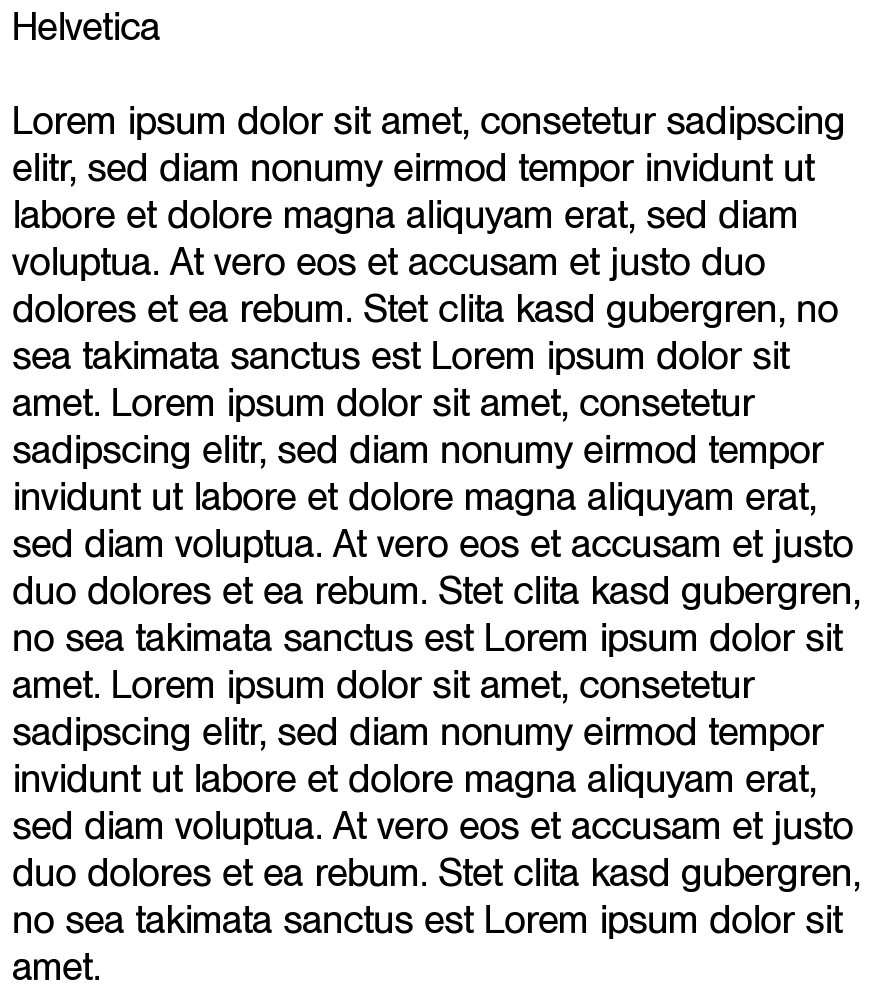
\includegraphics[width=.45\linewidth]{Lorem_Ipsum_Helvetica.png}
  \end{center}
  \caption{\label{fig:lorem} lorem ipsum rasterized plus a longish caption spanning two lines}
\end{figure}

Ut wisi enim ad minim veniam, quis nostrud exerci tation ullamcorper suscipit lobortis nisl ut aliquip ex ea commodo consequat. Duis autem vel eum iriure dolor in hendrerit in vulputate velit esse~\cite{Kindlmann1999}.

\subsection{Approaches to the Clustering-Problem}

Right of the start we had several ideas of how we could approach this problem. 
With the recent trend in machine learning we had a couple of ideas of how we could determine a similarity metric between two images or classify an image into a more usable vector of data.

We ended up using .... to determine the similarirty between two protein maps because we didnt manage to train a custom model in the given timeframe, due to .

But our initial results with a pretrained Imagenet \info{cite imagenet} \info{cite darknet publication} model let us to believe that it shoud be definetly possible for this specified task to find a machine learning solution. 

\subsection{Approaches to the Visualization-Task}

Our aproaches to visualizing the given clusters were the following, the reader is reminded that we are not just visualizing the clusters on a ''normal machine'' but rather the POWERWALL, a projected display with effectively 6-24 times the resolution of a consumer grade display. Details on the POWERWALL can be found \info{cite powerwall publicatoin here if available}.


\subsubsection{Ipsum}

\subsubsection{Dolor}

\begin{table}
\caption{
\label{tab:perf} lorem ipsum tabulated}
\centering
\vspace{0.3em}
\begin{tabular}{lrr}
dataset & full performance (fps) & half performance (ms)\\ \hline\\[-0.4em]
balls & 1,243 & 0.1 \\
buckets & 23 & 23 \\
bolts & 23,312,134.3 & 22.1 \\
\end{tabular}
\end{table}



%% if specified like this the section will be ommitted in review mode
\acknowledgments{
We would like to thank our supervisors M. Krone and F. Fries(?) as well as our project examiner Prof. ... . We are grateful for the experience and knowledge that working on this project has given us.
This work was partially funded by cake and cookies.
}

\bibliographystyle{abbrv}
%%use following if all content of bibtex file should be shown
%\nocite{*}
\bibliography{template}
\end{document} 
